\documentclass[11pt, letterpaper]{article}

% Fonts and Encoding
\usepackage[utf8]{inputenc}
\usepackage[T1]{fontenc}
\usepackage{lmodern} % High-quality Latin Modern vector font

% Math and Symbols
\usepackage{amsmath, amssymb, amsthm, amsfonts, mathrsfs, mathtools}

% Layout and Geometry
\usepackage{geometry}
\geometry{letterpaper, margin=1in}
\setlength{\parindent}{0pt}
\setlength{\parskip}{0.6em}

% Formatting and Graphics
\usepackage{graphicx, xcolor, enumitem, booktabs, array, tabularx}

% TikZ for Illustrations
\usepackage{tikz}
\usetikzlibrary{arrows.meta, positioning, shapes.geometric, calc, backgrounds, matrix}

% Clickable Links and TOC
\usepackage{hyperref}
\hypersetup{
    colorlinks=true,
    linkcolor=blue,
    filecolor=magenta,      
    urlcolor=cyan,
    pdftitle={Advanced Mathematics Topic},
}

% Theorem Environments
\newtheorem{theorem}{Theorem}[section]
\newtheorem{lemma}[theorem]{Lemma}
\newtheorem{proposition}[theorem]{Proposition}
\newtheorem{corollary}[theorem]{Corollary}
\theoremstyle{definition}
\newtheorem{definition}{Definition}[section]
\newtheorem{axiom}{Axiom}[section]
\newtheorem{example}{Example}[section]
\theoremstyle{remark}
\newtheorem{remark}{Remark}[section]

% Custom Commands (Enforced standard notation)
\newcommand{\R}{\mathbb{R}}
\newcommand{\N}{\mathbb{N}}
\newcommand{\Z}{\mathbb{Z}}
\newcommand{\Q}{\mathbb{Q}}
\newcommand{\E}{\mathbb{E}}
\newcommand{\Prob}{\mathbb{P}}
\newcommand{\F}{\mathcal{F}}

\title{\textbf{Mastery Guide: Diagonalization of Symmetric Matrices and Quadratic Forms}}
\author{Tashfeen Omran}
\date{\today}

\begin{document}

\maketitle
\tableofcontents
\newpage

\section{Part 1: Comprehensive Introduction, Context, and Prerequisites}

\subsection{Core Concepts}
The topic of \textbf{Diagonalization of Symmetric Matrices} and \textbf{Quadratic Forms} represents a profound intersection of algebra and geometry. 
A matrix $A$ is \textit{symmetric} if it equals its transpose, meaning $A^T = A$. The entries of a symmetric matrix are mirrored across its main diagonal. 
The central revelation of this topic is the \textbf{Spectral Theorem}, which states that every real symmetric matrix is not only diagonalizable but \textit{orthogonally} diagonalizable. This means we can find an orthonormal basis of eigenvectors for $\R^n$. 

A \textbf{Quadratic Form} is a scalar-valued function $Q(\mathbf{x}) = \mathbf{x}^T A \mathbf{x}$, where $A$ is a symmetric matrix. These forms generalize the concept of distance and energy, mapping a vector to a real number using pure quadratic terms (e.g., $x_1^2, x_2^2$) and cross-product terms (e.g., $x_1 x_2$).

\subsection{Intuition and Derivation}
Why are symmetric matrices so special? Geometrically, a symmetric matrix represents a linear transformation that scales space along mutually perpendicular axes. 
When we diagonalize a standard matrix $A = PDP^{-1}$, the columns of $P$ (the eigenvectors) form a skewed coordinate system. However, if $A$ is symmetric, the eigenvectors corresponding to distinct eigenvalues are naturally orthogonal. By normalizing these vectors, $P$ becomes an \textit{orthogonal matrix} (where $P^{-1} = P^T$). Thus, the diagonalization becomes $A = PDP^T$. This implies that applying $A$ is equivalent to rotating space ($P^T$), scaling along the standard axes ($D$), and rotating back ($P$).

\subsection{Historical Context and Motivation}
The study of symmetric matrices and quadratic forms originated in the 19th century with Augustin-Louis Cauchy and later David Hilbert. Cauchy was studying the principal axes of inertia in classical mechanics and the geometry of quadric surfaces (ellipsoids, hyperboloids). He discovered that the axes of these shapes are always mutually orthogonal, which mathematically translates to the Spectral Theorem for symmetric matrices. Later, this framework became the mathematical bedrock for Quantum Mechanics, where physical observables are represented by symmetric (or Hermitian) operators, and their real eigenvalues represent measurable quantities.

\subsection{Key Formulas}
\begin{itemize}
    \item \textbf{Orthogonal Matrix Property:} $P^{-1} = P^T \implies P^T P = I$.
    \item \textbf{Orthogonal Diagonalization:} $A = PDP^T$, where $D$ is diagonal and $P$ is orthogonal.
    \item \textbf{Spectral Decomposition:} $A = \lambda_1 \mathbf{u}_1 \mathbf{u}_1^T + \lambda_2 \mathbf{u}_2 \mathbf{u}_2^T + \dots + \lambda_n \mathbf{u}_n \mathbf{u}_n^T$.
    \item \textbf{Quadratic Form:} $Q(\mathbf{x}) = \mathbf{x}^T A \mathbf{x} = \sum_{i=1}^n \sum_{j=1}^n a_{ij} x_i x_j$.
\end{itemize}

\subsection{Prerequisites}
To master this topic, you must be fluent in:
\begin{enumerate}
    \item \textbf{Eigenvalues and Eigenvectors:} Solving $\det(A - \lambda I) = 0$ and finding the null space of $(A - \lambda I)$.
    \item \textbf{Dot Products and Orthogonality:} Computing $\mathbf{u} \cdot \mathbf{v} = \mathbf{u}^T \mathbf{v}$ and verifying $\mathbf{u} \cdot \mathbf{v} = 0$.
    \item \textbf{Gram-Schmidt Process:} Orthogonalizing a set of basis vectors, particularly when an eigenspace has a dimension greater than 1.
    \item \textbf{Matrix Transposition Rules:} Knowing that $(AB)^T = B^T A^T$.
\end{enumerate}

\newpage
\section{Part 2: Detailed Homework Solutions}
\textit{Note: A strategic selection of problems has been made to cover every distinct problem archetype present in the provided text, ensuring comprehensive conceptual coverage without redundant repetition.}

\renewcommand{\arraystretch}{1.5}
\begin{tabularx}{\textwidth}{>{\raggedright\arraybackslash}X}
\toprule
\textbf{Problem 1 (Exercise 1): Identify if the matrix is symmetric.} \\
$A = \begin{bmatrix} 4 & 3 \\ 3 & -8 \end{bmatrix}$ \\
\midrule
\textbf{Solution:} \\
A matrix $A$ is symmetric if $A^T = A$. We compute the transpose by swapping rows and columns:
\[ A^T = \begin{bmatrix} 4 & 3 \\ 3 & -8 \end{bmatrix}^T = \begin{bmatrix} 4 & 3 \\ 3 & -8 \end{bmatrix} \]
Since $A^T = A$, the matrix \textbf{is symmetric}. \\
\bottomrule
\end{tabularx}
\vspace{1em}

\begin{tabularx}{\textwidth}{>{\raggedright\arraybackslash}X}
\toprule
\textbf{Problem 2 (Exercise 4): Identify if the matrix is symmetric.} \\
$A = \begin{bmatrix} 1 & 3 & 5 \\ 3 & 1 & -6 \\ 5 & 4 & 1 \end{bmatrix}$ \\
\midrule
\textbf{Solution:} \\
We check if the entries across the main diagonal are equal, i.e., $A_{ij} = A_{ji}$ for all $i, j$.
Looking at the entry in row 2, column 3: $A_{23} = -6$.
Looking at the entry in row 3, column 2: $A_{32} = 4$.
Since $A_{23} \neq A_{32}$, $A^T \neq A$. The matrix \textbf{is not symmetric}. \\
\bottomrule
\end{tabularx}
\vspace{1em}

\begin{tabularx}{\textwidth}{>{\raggedright\arraybackslash}X}
\toprule
\textbf{Problem 3 (Exercise 7): Determine if the matrix is orthogonal. If orthogonal, find the inverse.} \\
$A = \begin{bmatrix} 1/\sqrt{2} & -1/\sqrt{2} \\ 1/\sqrt{2} & 1/\sqrt{2} \end{bmatrix}$ \\
\midrule
\textbf{Solution:} \\
A matrix is orthogonal if its columns form an orthonormal set. Let $\mathbf{c}_1$ and $\mathbf{c}_2$ be the columns of $A$.
1. Check if they are orthogonal:
\[ \mathbf{c}_1 \cdot \mathbf{c}_2 = \left(\frac{1}{\sqrt{2}}\right)\left(-\frac{1}{\sqrt{2}}\right) + \left(\frac{1}{\sqrt{2}}\right)\left(\frac{1}{\sqrt{2}}\right) = -\frac{1}{2} + \frac{1}{2} = 0 \]
2. Check if they are unit vectors:
\[ \|\mathbf{c}_1\|^2 = \left(\frac{1}{\sqrt{2}}\right)^2 + \left(\frac{1}{\sqrt{2}}\right)^2 = \frac{1}{2} + \frac{1}{2} = 1 \]
\[ \|\mathbf{c}_2\|^2 = \left(-\frac{1}{\sqrt{2}}\right)^2 + \left(\frac{1}{\sqrt{2}}\right)^2 = \frac{1}{2} + \frac{1}{2} = 1 \]
Since the columns are orthonormal, $A$ \textbf{is an orthogonal matrix}. 
For an orthogonal matrix, $A^{-1} = A^T$. Therefore:
\[ A^{-1} = \begin{bmatrix} 1/\sqrt{2} & 1/\sqrt{2} \\ -1/\sqrt{2} & 1/\sqrt{2} \end{bmatrix} \] \\
\bottomrule
\end{tabularx}
\vspace{1em}

\begin{tabularx}{\textwidth}{>{\raggedright\arraybackslash}X}
\toprule
\textbf{Problem 4 (Exercise 10): Determine if the matrix is orthogonal. If orthogonal, find the inverse.} \\
$A = \begin{bmatrix} 2/3 & 1/3 & -2/3 \\ -2/3 & 2/3 & -1/3 \\ 1/3 & 2/3 & 2/3 \end{bmatrix}$ \\
\midrule
\textbf{Solution:} \\
We can verify orthogonality by checking if $A^T A = I$.
\[ A^T A = \begin{bmatrix} 2/3 & -2/3 & 1/3 \\ 1/3 & 2/3 & 2/3 \\ -2/3 & -1/3 & 2/3 \end{bmatrix} \begin{bmatrix} 2/3 & 1/3 & -2/3 \\ -2/3 & 2/3 & -1/3 \\ 1/3 & 2/3 & 2/3 \end{bmatrix} \]
Let's compute the diagonal entries (dot products of columns with themselves):
Row 1 $\cdot$ Col 1: $(2/3)^2 + (-2/3)^2 + (1/3)^2 = (4+4+1)/9 = 1$.
Row 2 $\cdot$ Col 2: $(1/3)^2 + (2/3)^2 + (2/3)^2 = (1+4+4)/9 = 1$.
Row 3 $\cdot$ Col 3: $(-2/3)^2 + (-1/3)^2 + (2/3)^2 = (4+1+4)/9 = 1$.
Now compute the off-diagonal entries (dot products of distinct columns):
Row 1 $\cdot$ Col 2: $(2/3)(1/3) + (-2/3)(2/3) + (1/3)(2/3) = (2 - 4 + 2)/9 = 0$.
Row 1 $\cdot$ Col 3: $(2/3)(-2/3) + (-2/3)(-1/3) + (1/3)(2/3) = (-4 + 2 + 2)/9 = 0$.
Row 2 $\cdot$ Col 3: $(1/3)(-2/3) + (2/3)(-1/3) + (2/3)(2/3) = (-2 - 2 + 4)/9 = 0$.
Since $A^T A = I$, $A$ \textbf{is an orthogonal matrix}.
The inverse is simply the transpose:
\[ A^{-1} = A^T = \begin{bmatrix} 2/3 & -2/3 & 1/3 \\ 1/3 & 2/3 & 2/3 \\ -2/3 & -1/3 & 2/3 \end{bmatrix} \] \\
\bottomrule
\end{tabularx}
\vspace{1em}

\begin{tabularx}{\textwidth}{>{\raggedright\arraybackslash}X}
\toprule
\textbf{Problem 5 (Exercise 13): Orthogonally diagonalize the matrix, giving an orthogonal matrix $P$ and a diagonal matrix $D$.} \\
$A = \begin{bmatrix} 4 & 1 \\ 1 & 4 \end{bmatrix}$ \\
\midrule
\textbf{Solution:} \\
\textbf{Step 1: Find the eigenvalues.}
The characteristic equation is $\det(A - \lambda I) = 0$:
\[ \det \begin{bmatrix} 4-\lambda & 1 \\ 1 & 4-\lambda \end{bmatrix} = (4-\lambda)^2 - 1 = \lambda^2 - 8\lambda + 16 - 1 = \lambda^2 - 8\lambda + 15 = 0 \]
Factoring yields $(\lambda - 5)(\lambda - 3) = 0$. The eigenvalues are $\lambda_1 = 5$ and $\lambda_2 = 3$.

\textbf{Step 2: Find the eigenvectors.}
For $\lambda_1 = 5$:
\[ A - 5I = \begin{bmatrix} -1 & 1 \\ 1 & -1 \end{bmatrix} \xrightarrow{\text{RREF}} \begin{bmatrix} 1 & -1 \\ 0 & 0 \end{bmatrix} \]
The eigenvector is $\mathbf{v}_1 = \begin{bmatrix} 1 \\ 1 \end{bmatrix}$.

For $\lambda_2 = 3$:
\[ A - 3I = \begin{bmatrix} 1 & 1 \\ 1 & 1 \end{bmatrix} \xrightarrow{\text{RREF}} \begin{bmatrix} 1 & 1 \\ 0 & 0 \end{bmatrix} \]
The eigenvector is $\mathbf{v}_2 = \begin{bmatrix} -1 \\ 1 \end{bmatrix}$.

\textbf{Step 3: Normalize the eigenvectors.}
Since $A$ is symmetric and the eigenvalues are distinct, $\mathbf{v}_1$ and $\mathbf{v}_2$ are already orthogonal ($\mathbf{v}_1 \cdot \mathbf{v}_2 = -1 + 1 = 0$). We just need to normalize them to create an orthonormal basis.
\[ \|\mathbf{v}_1\| = \sqrt{1^2 + 1^2} = \sqrt{2} \implies \mathbf{u}_1 = \begin{bmatrix} 1/\sqrt{2} \\ 1/\sqrt{2} \end{bmatrix} \]
\[ \|\mathbf{v}_2\| = \sqrt{(-1)^2 + 1^2} = \sqrt{2} \implies \mathbf{u}_2 = \begin{bmatrix} -1/\sqrt{2} \\ 1/\sqrt{2} \end{bmatrix} \]

\textbf{Step 4: Construct $P$ and $D$.}
\[ P = \begin{bmatrix} 1/\sqrt{2} & -1/\sqrt{2} \\ 1/\sqrt{2} & 1/\sqrt{2} \end{bmatrix}, \quad D = \begin{bmatrix} 5 & 0 \\ 0 & 3 \end{bmatrix} \] \\
\bottomrule
\end{tabularx}
\vspace{1em}

\begin{tabularx}{\textwidth}{>{\raggedright\arraybackslash}X}
\toprule
\textbf{Problem 6 (Exercise 17): Orthogonally diagonalize the matrix. (Eigenvalues are $-5, 5, 8$)} \\
$A = \begin{bmatrix} 1 & 1 & 6 \\ 1 & 6 & 1 \\ 6 & 1 & 1 \end{bmatrix}$ \\
\midrule
\textbf{Solution:} \\
\textbf{Step 1: Find eigenvectors for $\lambda = 8$.}
\[ A - 8I = \begin{bmatrix} -7 & 1 & 6 \\ 1 & -2 & 1 \\ 6 & 1 & -7 \end{bmatrix} \]
Row operations: Swap $R_1$ and $R_2$, then eliminate down:
\[ \begin{bmatrix} 1 & -2 & 1 \\ -7 & 1 & 6 \\ 6 & 1 & -7 \end{bmatrix} \xrightarrow{R_2+7R_1, R_3-6R_1} \begin{bmatrix} 1 & -2 & 1 \\ 0 & -13 & 13 \\ 0 & 13 & -13 \end{bmatrix} \xrightarrow{\text{RREF}} \begin{bmatrix} 1 & 0 & -1 \\ 0 & 1 & -1 \\ 0 & 0 & 0 \end{bmatrix} \]
This gives $x_1 = x_3$ and $x_2 = x_3$. The eigenvector is $\mathbf{v}_1 = \begin{bmatrix} 1 \\ 1 \\ 1 \end{bmatrix}$.
Normalizing: $\|\mathbf{v}_1\| = \sqrt{3} \implies \mathbf{u}_1 = \begin{bmatrix} 1/\sqrt{3} \\ 1/\sqrt{3} \\ 1/\sqrt{3} \end{bmatrix}$.

\textbf{Step 2: Find eigenvectors for $\lambda = 5$.}
\[ A - 5I = \begin{bmatrix} -4 & 1 & 6 \\ 1 & 1 & 1 \\ 6 & 1 & -4 \end{bmatrix} \]
Swap $R_1$ and $R_2$, then eliminate down:
\[ \begin{bmatrix} 1 & 1 & 1 \\ -4 & 1 & 6 \\ 6 & 1 & -4 \end{bmatrix} \xrightarrow{R_2+4R_1, R_3-6R_1} \begin{bmatrix} 1 & 1 & 1 \\ 0 & 5 & 10 \\ 0 & -5 & -10 \end{bmatrix} \xrightarrow{\text{RREF}} \begin{bmatrix} 1 & 0 & -1 \\ 0 & 1 & 2 \\ 0 & 0 & 0 \end{bmatrix} \]
This gives $x_1 = x_3$ and $x_2 = -2x_3$. The eigenvector is $\mathbf{v}_2 = \begin{bmatrix} 1 \\ -2 \\ 1 \end{bmatrix}$.
Normalizing: $\|\mathbf{v}_2\| = \sqrt{1+4+1} = \sqrt{6} \implies \mathbf{u}_2 = \begin{bmatrix} 1/\sqrt{6} \\ -2/\sqrt{6} \\ 1/\sqrt{6} \end{bmatrix}$.

\textbf{Step 3: Find eigenvectors for $\lambda = -5$.}
\[ A + 5I = \begin{bmatrix} 6 & 1 & 6 \\ 1 & 11 & 1 \\ 6 & 1 & 6 \end{bmatrix} \]
Swap $R_1$ and $R_2$, then eliminate down:
\[ \begin{bmatrix} 1 & 11 & 1 \\ 6 & 1 & 6 \\ 6 & 1 & 6 \end{bmatrix} \xrightarrow{R_2-6R_1, R_3-6R_1} \begin{bmatrix} 1 & 11 & 1 \\ 0 & -65 & 0 \\ 0 & -65 & 0 \end{bmatrix} \xrightarrow{\text{RREF}} \begin{bmatrix} 1 & 0 & 1 \\ 0 & 1 & 0 \\ 0 & 0 & 0 \end{bmatrix} \]
This gives $x_1 = -x_3$ and $x_2 = 0$. The eigenvector is $\mathbf{v}_3 = \begin{bmatrix} -1 \\ 0 \\ 1 \end{bmatrix}$.
Normalizing: $\|\mathbf{v}_3\| = \sqrt{1+0+1} = \sqrt{2} \implies \mathbf{u}_3 = \begin{bmatrix} -1/\sqrt{2} \\ 0 \\ 1/\sqrt{2} \end{bmatrix}$.

\textbf{Step 4: Construct $P$ and $D$.}
\[ P = \begin{bmatrix} 1/\sqrt{3} & 1/\sqrt{6} & -1/\sqrt{2} \\ 1/\sqrt{3} & -2/\sqrt{6} & 0 \\ 1/\sqrt{3} & 1/\sqrt{6} & 1/\sqrt{2} \end{bmatrix}, \quad D = \begin{bmatrix} 8 & 0 & 0 \\ 0 & 5 & 0 \\ 0 & 0 & -5 \end{bmatrix} \] \\
\bottomrule
\end{tabularx}
\vspace{1em}

\begin{tabularx}{\textwidth}{>{\raggedright\arraybackslash}X}
\toprule
\textbf{Problem 7 (Exercise 25 \& 26): True or False.} \\
25. An $n \times n$ matrix that is orthogonally diagonalizable must be symmetric. \\
26. There are symmetric matrices that are not orthogonally diagonalizable. \\
\midrule
\textbf{Solution:} \\
\textbf{25. True.} By Theorem 2 in the text, an $n \times n$ matrix $A$ is orthogonally diagonalizable if and only if $A$ is a symmetric matrix. If $A = PDP^T$, then $A^T = (PDP^T)^T = (P^T)^T D^T P^T = PDP^T = A$. \\
\textbf{26. False.} The Spectral Theorem (Theorem 3) guarantees that \textit{every} real symmetric matrix is orthogonally diagonalizable. There are no exceptions in the real numbers. \\
\bottomrule
\end{tabularx}
\vspace{1em}

\begin{tabularx}{\textwidth}{>{\raggedright\arraybackslash}X}
\toprule
\textbf{Problem 8 (Exercise 33): Proof.} \\
Show that if $A$ is an $n \times n$ symmetric matrix, then $(A\mathbf{x}) \cdot \mathbf{y} = \mathbf{x} \cdot (A\mathbf{y})$ for all $\mathbf{x}, \mathbf{y}$ in $\R^n$. \\
\midrule
\textbf{Solution:} \\
Recall that the dot product of two column vectors $\mathbf{u}$ and $\mathbf{v}$ can be written as a matrix multiplication: $\mathbf{u} \cdot \mathbf{v} = \mathbf{u}^T \mathbf{v}$.
Applying this to the left side of the equation:
\[ (A\mathbf{x}) \cdot \mathbf{y} = (A\mathbf{x})^T \mathbf{y} \]
Using the property of transposes $(AB)^T = B^T A^T$, we get:
\[ (A\mathbf{x})^T \mathbf{y} = (\mathbf{x}^T A^T) \mathbf{y} \]
Since $A$ is a symmetric matrix, we know $A^T = A$. Substituting this in:
\[ (\mathbf{x}^T A) \mathbf{y} = \mathbf{x}^T (A\mathbf{y}) \]
Converting back to dot product notation:
\[ \mathbf{x}^T (A\mathbf{y}) = \mathbf{x} \cdot (A\mathbf{y}) \]
Thus, $(A\mathbf{x}) \cdot \mathbf{y} = \mathbf{x} \cdot (A\mathbf{y})$. \qed \\
\bottomrule
\end{tabularx}

\newpage
\section{Part 3: In-Depth Analysis of Problems and Techniques}

\subsection{A) Problem Types and General Approach}
\begin{itemize}
    \item \textbf{Type 1: Matrix Identification (Symmetric/Orthogonal):} These problems require applying definitions. For symmetry, check if $A = A^T$. For orthogonality, check if $A^T A = I$. The strategy is pure matrix multiplication and observation.
    \item \textbf{Type 2: Orthogonal Diagonalization:} This is the core algorithmic problem of the chapter. 
    \begin{enumerate}
        \item Find eigenvalues via $\det(A - \lambda I) = 0$.
        \item Find a basis for each eigenspace via $\text{Nul}(A - \lambda I)$.
        \item \textit{Crucial Step:} If an eigenspace has dimension $> 1$, use the Gram-Schmidt process to ensure the basis vectors are orthogonal. (If eigenvalues are distinct, eigenvectors are automatically orthogonal).
        \item Normalize all eigenvectors to length 1.
        \item Assemble $P$ (columns are the normalized eigenvectors) and $D$ (diagonal entries are eigenvalues).
    \end{enumerate}
    \item \textbf{Type 3: Theoretical Proofs:} These rely heavily on the properties of transposes: $(AB)^T = B^T A^T$, $(A^T)^T = A$, and the translation of dot products into matrix multiplication $\mathbf{u} \cdot \mathbf{v} = \mathbf{u}^T \mathbf{v}$.
\end{itemize}

\subsection{B) Key Algebraic and Calculus Manipulations}
\begin{itemize}
    \item \textbf{The Dot Product Translation:} Used in Problem 8. Converting $\mathbf{u} \cdot \mathbf{v}$ to $\mathbf{u}^T \mathbf{v}$ is the most powerful algebraic trick in linear algebra for proving properties about symmetric matrices. It allows matrix algebra rules (like associativity) to be applied to geometric concepts (like orthogonality).
    \item \textbf{Vector Normalization:} Used in Problems 5 and 6. Dividing a vector by its magnitude $\mathbf{u} = \mathbf{v} / \|\mathbf{v}\|$ is mandatory. A common pitfall is finding orthogonal eigenvectors but forgetting to normalize them, which results in a $P$ matrix that is invertible but \textit{not} orthogonal.
    \item \textbf{Row Reduction (RREF) for Null Spaces:} Used extensively in finding eigenvectors. The trick is to recognize that $A - \lambda I$ will \textit{always} have at least one row of zeros if $\lambda$ is a true eigenvalue. If it doesn't, you made an arithmetic error in finding $\lambda$.
\end{itemize}

\newpage
\section{Part 4: "Cheatsheet" and Tips for Success}

\subsection{Summary of Important Formulas}
\begin{itemize}
    \item \textbf{Symmetric Matrix:} $A^T = A$
    \item \textbf{Orthogonal Matrix:} $P^T P = I \implies P^{-1} = P^T$
    \item \textbf{Orthogonal Diagonalization:} $A = P D P^T$
    \item \textbf{Spectral Decomposition:} $A = \sum_{i=1}^n \lambda_i \mathbf{u}_i \mathbf{u}_i^T$
    \item \textbf{Quadratic Form:} $Q(\mathbf{x}) = \mathbf{x}^T A \mathbf{x}$
\end{itemize}

\subsection{Cheats, Tricks, and Shortcuts}
\begin{itemize}
    \item \textbf{The Orthogonality Check (Cheat):} When you find eigenvectors for distinct eigenvalues of a symmetric matrix, take their dot product immediately. If it is not exactly zero, you made an algebra mistake. This is a built-in error-checking mechanism!
    \item \textbf{The $2 \times 2$ Eigenvalue Shortcut:} For a $2 \times 2$ matrix, the characteristic equation is always $\lambda^2 - \text{tr}(A)\lambda + \det(A) = 0$. Use this to bypass the determinant setup.
    \item \textbf{Quadratic Form Matrix Construction:} To build the symmetric matrix $A$ from a quadratic form equation, put the coefficients of the squared terms ($x_i^2$) on the main diagonal. For any cross term $c x_i x_j$, divide the coefficient $c$ by 2 and place it in both the $(i,j)$ and $(j,i)$ positions of the matrix.
\end{itemize}

\subsection{Common Pitfalls}
\begin{itemize}
    \item \textbf{Forgetting Gram-Schmidt:} If an eigenvalue has a multiplicity of 2 (e.g., $\lambda = 7, 7$), you will get two eigenvectors. They are \textit{not} guaranteed to be orthogonal to each other. You MUST apply Gram-Schmidt to these two vectors before normalizing.
    \item \textbf{Forgetting to Normalize:} $P$ must consist of \textit{orthonormal} vectors, not just orthogonal ones. If you don't divide by the magnitude, $P^T P \neq I$.
\end{itemize}

\vspace{2em}
\begin{center}
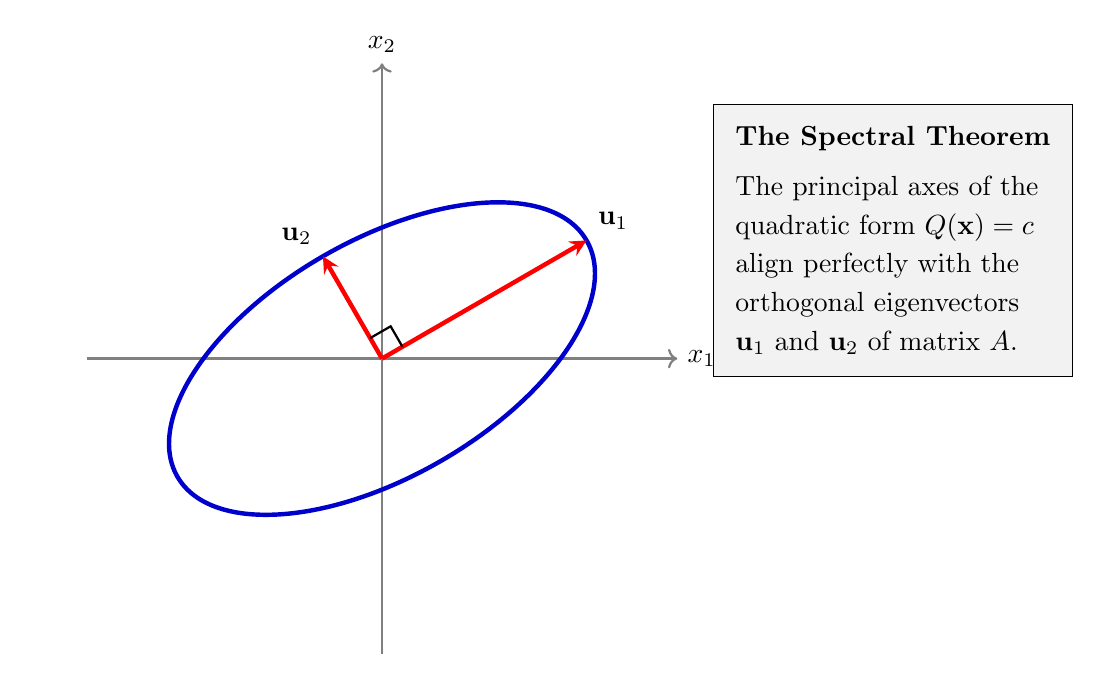
\begin{tikzpicture}[scale=1.5]
    % Background to ensure clean rendering
    \fill[white] (-3,-2.5) rectangle (4.5,2.5);
    
    % Axes
    \draw[thick, ->, gray] (-2.5,0) -- (2.5,0) node[right, text=black] {$x_1$};
    \draw[thick, ->, gray] (0,-2.5) -- (0,2.5) node[above, text=black] {$x_2$};
    
    % Ellipse representing a quadratic form x^T A x = c
    \draw[ultra thick, blue!80!black, rotate=30] (0,0) ellipse (2cm and 1cm);
    
    % Eigenvectors (Principal Axes)
    \draw[->, ultra thick, red, >=stealth] (0,0) -- (1.732, 1) node[above right, text=black] {$\mathbf{u}_1$};
    \draw[->, ultra thick, red, >=stealth] (0,0) -- (-0.5, 0.866) node[above left, text=black] {$\mathbf{u}_2$};
    
    % Right angle symbol
    \draw[thick, rotate=30] (0.2,0) -- (0.2,0.2) -- (0,0.2);
    
    % Legend using single-node multiline rule
    \node[align=left, inner sep=8pt, anchor=west, draw, fill=gray!10] at (2.8, 1) {
        \textbf{The Spectral Theorem} \\[6pt]
        The principal axes of the \\[2pt]
        quadratic form $Q(\mathbf{x}) = c$ \\[2pt]
        align perfectly with the \\[2pt]
        orthogonal eigenvectors \\[2pt]
        $\mathbf{u}_1$ and $\mathbf{u}_2$ of matrix $A$.
    };
\end{tikzpicture}
\end{center}

\newpage
\section{Part 5: Conceptual Synthesis and The "Big Picture"}

\subsection{A) Thematic Connections}
The overarching theme of this topic is \textbf{Change of Basis to Reveal Inherent Structure}. In earlier chapters, we learned that multiplying a vector by a matrix can be messy—it skews, rotates, and stretches space simultaneously. Diagonalization was our first attempt to find a "good" coordinate system where the matrix just acts as a simple scaling operation. 

Symmetric matrices represent the pinnacle of this theme. Because their eigenvectors are orthogonal, the "good" coordinate system is just a rigid rotation of our standard Cartesian axes. We don't have to warp or skew space to understand the matrix; we just have to look at it from the right angle. This connects deeply to the concept of \textit{Principal Component Analysis (PCA)} in statistics, where we rotate our view of a dataset to align with the axes of maximum variance.

\subsection{B) Forward and Backward Links}
\textbf{Backward Links:} This topic relies heavily on the Gram-Schmidt process (Chapter 6) and basic eigenvalue theory (Chapter 5). It is the ultimate payoff for learning about orthogonal projections. \\
\textbf{Forward Links:} Orthogonal diagonalization is the direct prerequisite for the \textbf{Singular Value Decomposition (SVD)}. While the Spectral Theorem only applies to square, symmetric matrices, SVD extends this geometric intuition (rotation $\to$ scaling $\to$ rotation) to \textit{any} $m \times n$ matrix. Furthermore, understanding Quadratic Forms is the bedrock for Multivariable Calculus (specifically the Second Derivative Test for finding local minima/maxima using the Hessian matrix, which is always symmetric).

\section{Part 6: Abstract Real-World Modeling (AI, ML, \& Quant Finance)}

\subsection{A) Concrete Scenarios}
\begin{enumerate}
    \item \textbf{Machine Learning (Principal Component Analysis):} In ML, high-dimensional data is often reduced using PCA. The covariance matrix of the data is always symmetric. By orthogonally diagonalizing this covariance matrix, the eigenvectors (principal components) provide a new orthogonal basis that captures the most variance, allowing for dimensionality reduction without massive information loss.
    \item \textbf{Quantitative Finance (Portfolio Optimization):} In Modern Portfolio Theory (Markowitz), the risk of a portfolio is modeled as the variance of its returns. This variance is calculated using a quadratic form $\mathbf{w}^T \Sigma \mathbf{w}$, where $\mathbf{w}$ is the vector of asset weights and $\Sigma$ is the symmetric covariance matrix of asset returns.
\end{enumerate}

\subsection{B) Model Problem Setup: Markowitz Portfolio Optimization}
Let us rigorously define the optimization problem for a quantitative hedge fund looking to minimize risk for a target expected return.

\textbf{State Space and Variables:}
Let $N$ be the number of available assets.
Let $\mathbf{w} \in \R^N$ be the portfolio weight vector, where $w_i$ is the fraction of capital allocated to asset $i$.
Let $\boldsymbol{\mu} \in \R^N$ be the vector of expected returns for each asset.
Let $\Sigma \in \R^{N \times N}$ be the covariance matrix of the asset returns. By definition, $\Sigma$ is symmetric ($\Sigma^T = \Sigma$) and positive semi-definite ($\mathbf{x}^T \Sigma \mathbf{x} \geq 0$ for all $\mathbf{x}$).

\textbf{The Objective:}
The expected return of the portfolio is a linear combination: $E[R_p] = \mathbf{w}^T \boldsymbol{\mu}$.
The variance (risk) of the portfolio is a quadratic form: $\text{Var}(R_p) = \mathbf{w}^T \Sigma \mathbf{w}$.

The fund manager seeks to minimize the portfolio variance subject to achieving a target expected return $\mu_{target}$, and ensuring all capital is deployed (weights sum to 1).

\textbf{Mathematical Formulation:}
\[ \min_{\mathbf{w}} \quad \frac{1}{2} \mathbf{w}^T \Sigma \mathbf{w} \]
\[ \text{subject to} \quad \mathbf{w}^T \boldsymbol{\mu} = \mu_{target} \]
\[ \quad \mathbf{w}^T \mathbf{1} = 1 \]

This is a constrained quadratic programming problem. Because $\Sigma$ is symmetric, we can use the method of Lagrange multipliers. The Lagrangian is:
\[ \mathcal{L}(\mathbf{w}, \lambda_1, \lambda_2) = \frac{1}{2} \mathbf{w}^T \Sigma \mathbf{w} - \lambda_1 (\mathbf{w}^T \boldsymbol{\mu} - \mu_{target}) - \lambda_2 (\mathbf{w}^T \mathbf{1} - 1) \]
Taking the gradient with respect to $\mathbf{w}$ and setting it to zero yields:
\[ \nabla_{\mathbf{w}} \mathcal{L} = \Sigma \mathbf{w} - \lambda_1 \boldsymbol{\mu} - \lambda_2 \mathbf{1} = \mathbf{0} \implies \mathbf{w} = \Sigma^{-1} (\lambda_1 \boldsymbol{\mu} + \lambda_2 \mathbf{1}) \]
This elegant closed-form solution for the optimal trading weights is only possible because the derivative of the quadratic form $\frac{1}{2}\mathbf{w}^T \Sigma \mathbf{w}$ simplifies perfectly to $\Sigma \mathbf{w}$, a direct consequence of $\Sigma$ being symmetric.

\newpage
\section{Part 7: Common Variations and Untested Concepts}

\subsection{Positive Definite Matrices and Sylvester's Criterion}
While the homework covers translating a matrix into a quadratic form, it does not test the \textit{classification} of quadratic forms. A symmetric matrix $A$ is \textbf{positive definite} if its quadratic form $Q(\mathbf{x}) = \mathbf{x}^T A \mathbf{x} > 0$ for all $\mathbf{x} \neq \mathbf{0}$. This is crucial in optimization (ensuring a critical point is a minimum).

\textbf{Untested Concept Example:} Determine if $A = \begin{bmatrix} 3 & 1 \\ 1 & 2 \end{bmatrix}$ is positive definite.

\textbf{Method 1: Eigenvalues.} A matrix is positive definite if and only if all its eigenvalues are strictly positive.
$\det(A - \lambda I) = (3-\lambda)(2-\lambda) - 1 = \lambda^2 - 5\lambda + 5 = 0$.
Using the quadratic formula: $\lambda = \frac{5 \pm \sqrt{25 - 20}}{2} = \frac{5 \pm \sqrt{5}}{2}$. Both eigenvalues are positive, so $A$ is positive definite.

\textbf{Method 2: Sylvester's Criterion.} A matrix is positive definite if and only if all its leading principal minors (determinants of upper-left submatrices) are positive.
1st minor: $\det([3]) = 3 > 0$.
2nd minor: $\det(A) = (3)(2) - (1)(1) = 5 > 0$.
Since both are positive, $A$ is positive definite. This method is often much faster than finding eigenvalues!

\section{Part 8: Advanced Diagnostic Testing: "Find the Flaw"}
\textit{Below are five problems with complete solutions. However, each solution contains a single, critical flaw. Your task is to act as the grader: identify the error, explain why it is wrong in one sentence, and provide the correct final step.}

\vspace{1em}
\textbf{Problem 1:} Orthogonally diagonalize $A = \begin{bmatrix} 2 & 1 \\ 1 & 2 \end{bmatrix}$.
\textit{Flawed Solution:}
The eigenvalues are $\lambda_1 = 3$ and $\lambda_2 = 1$.
For $\lambda_1 = 3$, $A - 3I = \begin{bmatrix} -1 & 1 \\ 1 & -1 \end{bmatrix} \implies \mathbf{v}_1 = \begin{bmatrix} 1 \\ 1 \end{bmatrix}$.
For $\lambda_2 = 1$, $A - I = \begin{bmatrix} 1 & 1 \\ 1 & 1 \end{bmatrix} \implies \mathbf{v}_2 = \begin{bmatrix} -1 \\ 1 \end{bmatrix}$.
Therefore, $P = \begin{bmatrix} 1 & -1 \\ 1 & 1 \end{bmatrix}$ and $D = \begin{bmatrix} 3 & 0 \\ 0 & 1 \end{bmatrix}$.

\textbf{Problem 2:} Write the spectral decomposition of a symmetric matrix $A$ with orthogonal eigenvectors $\mathbf{u}_1, \mathbf{u}_2$ and eigenvalues $\lambda_1, \lambda_2$.
\textit{Flawed Solution:}
By the spectral theorem, the matrix can be broken down into rank-1 pieces based on its spectrum. The decomposition is:
$A = \lambda_1 \mathbf{u}_1^T \mathbf{u}_1 + \lambda_2 \mathbf{u}_2^T \mathbf{u}_2$.

\textbf{Problem 3:} Find the quadratic form $Q(\mathbf{x})$ associated with the matrix $A = \begin{bmatrix} 1 & 4 \\ 0 & 1 \end{bmatrix}$.
\textit{Flawed Solution:}
The quadratic form is given by $Q(\mathbf{x}) = \mathbf{x}^T A \mathbf{x}$.
$Q(\mathbf{x}) = \begin{bmatrix} x_1 & x_2 \end{bmatrix} \begin{bmatrix} 1 & 4 \\ 0 & 1 \end{bmatrix} \begin{bmatrix} x_1 \\ x_2 \end{bmatrix} = x_1^2 + 4x_1 x_2 + x_2^2$.

\textbf{Problem 4:} An eigenspace for $\lambda = 4$ has basis vectors $\mathbf{v}_1 = \begin{bmatrix} 1 \\ 1 \\ 0 \end{bmatrix}$ and $\mathbf{v}_2 = \begin{bmatrix} 1 \\ 0 \\ 1 \end{bmatrix}$. Find an orthogonal basis for this eigenspace using Gram-Schmidt.
\textit{Flawed Solution:}
Let $\mathbf{z}_1 = \mathbf{v}_1$.
To find $\mathbf{z}_2$, we subtract the projection of $\mathbf{v}_2$ onto $\mathbf{z}_1$:
$\mathbf{z}_2 = \mathbf{v}_2 - \frac{\mathbf{v}_2 \cdot \mathbf{z}_1}{\mathbf{v}_2 \cdot \mathbf{v}_2} \mathbf{z}_1 = \begin{bmatrix} 1 \\ 0 \\ 1 \end{bmatrix} - \frac{1}{2} \begin{bmatrix} 1 \\ 1 \\ 0 \end{bmatrix} = \begin{bmatrix} 1/2 \\ -1/2 \\ 1 \end{bmatrix}$.

\textbf{Problem 5:} If $A$ is a symmetric matrix with eigenvalue $\lambda = 5$ and corresponding eigenvector $\mathbf{v}$, what is the eigenvalue of $A^2$ corresponding to $\mathbf{v}$?
\textit{Flawed Solution:}
Since $A$ is symmetric, $A^2$ is also symmetric. The eigenvectors remain the same, and because the matrix is squared, the eigenvalue remains $\lambda = 5$ because scalar multiples of eigenvectors don't change the spectrum.

\vspace{2em}
\hrule
\vspace{1em}
\textbf{Grader's Key (Corrections):}

\textbf{Correction 1:} The flaw is that the eigenvectors were not normalized to length 1, meaning $P$ is not an orthogonal matrix ($P^T P \neq I$). 
\textit{Correct Step:} Divide by $\sqrt{2}$. $P = \begin{bmatrix} 1/\sqrt{2} & -1/\sqrt{2} \\ 1/\sqrt{2} & 1/\sqrt{2} \end{bmatrix}$.

\textbf{Correction 2:} The flaw is writing the outer product backwards; $\mathbf{u}_i^T \mathbf{u}_i$ results in a scalar (the dot product), whereas $\mathbf{u}_i \mathbf{u}_i^T$ results in an $n \times n$ rank-1 matrix.
\textit{Correct Step:} $A = \lambda_1 \mathbf{u}_1 \mathbf{u}_1^T + \lambda_2 \mathbf{u}_2 \mathbf{u}_2^T$.

\textbf{Correction 3:} The flaw is applying the quadratic form definition to a non-symmetric matrix; the matrix of a quadratic form must be symmetric, so the off-diagonal entries must be averaged.
\textit{Correct Step:} The symmetric matrix for this form is $A = \begin{bmatrix} 1 & 2 \\ 2 & 1 \end{bmatrix}$.

\textbf{Correction 4:} The flaw is in the denominator of the Gram-Schmidt projection formula; it should be divided by $\mathbf{z}_1 \cdot \mathbf{z}_1$, not $\mathbf{v}_2 \cdot \mathbf{v}_2$.
\textit{Correct Step:} $\mathbf{z}_2 = \mathbf{v}_2 - \frac{\mathbf{v}_2 \cdot \mathbf{z}_1}{\mathbf{z}_1 \cdot \mathbf{z}_1} \mathbf{z}_1 = \begin{bmatrix} 1 \\ 0 \\ 1 \end{bmatrix} - \frac{1}{2} \begin{bmatrix} 1 \\ 1 \\ 0 \end{bmatrix} = \begin{bmatrix} 1/2 \\ -1/2 \\ 1 \end{bmatrix}$. (The numerical answer happened to be the same because $\|\mathbf{v}_2\|^2 = \|\mathbf{z}_1\|^2 = 2$, but the formula used was conceptually flawed).

\textbf{Correction 5:} The flaw is claiming the eigenvalue remains the same; if $A\mathbf{v} = \lambda\mathbf{v}$, then $A^2\mathbf{v} = A(A\mathbf{v}) = A(\lambda\mathbf{v}) = \lambda(A\mathbf{v}) = \lambda^2\mathbf{v}$.
\textit{Correct Step:} The eigenvalue of $A^2$ is $\lambda^2 = 25$.

\end{document}